\documentclass[12pt,letterpaper]{article}
\usepackage[utf8]{inputenc}
\usepackage{listings, float, xcolor}

%----- Configuración del estilo del documento------%
\usepackage{graphicx, fancyhdr}
\usepackage{enumitem, pifont, hyperref, ulem, tabularx}
\usepackage[left=2cm,right=2cm,top=1.8cm,bottom=2.3cm]{geometry}


%------ Paquetes matemáticos básicos --------%
\usepackage{amsmath, amssymb, amsthm}

\renewcommand{\lstlistingname}{Código}

%------ Definimos los colores para la sintaxis del código --------%
\definecolor{keywordcolor}{rgb}{0.5, 0.0, 0.5}  % Morado para palabras clave
\definecolor{commentcolor}{rgb}{0.25, 0.5, 0.35} % Verde para comentarios
\definecolor{stringcolor}{rgb}{0.88, 0.68, 0.18}  % Mostaza anaranjado para los strings
\definecolor{backgroundcolor}{rgb}{0.95, 0.95, 0.95} % Gris claro para fondo

%------ Configuración para mostrar código en C++ --------%
\lstdefinestyle{cppstyle}{
  language=C++,
  basicstyle=\ttfamily\footnotesize,
  keywordstyle=\color{keywordcolor}\bfseries,
  commentstyle=\color{commentcolor},
  stringstyle=\color{stringcolor},
  numbers=left,
  numberstyle=\tiny,
  stepnumber=1,
  numbersep=8pt,
  backgroundcolor=\color{backgroundcolor},
  tabsize=2,
  showspaces=false,
  showstringspaces=false,
  breaklines=true,
  frame=single,
  captionpos=b
}

\begin{document}

%------ Encabezado -------- %
\hrule height 0.1pt
\bigskip
\begin{center}
  \begin{minipage}{3cm}
    \begin{center}
      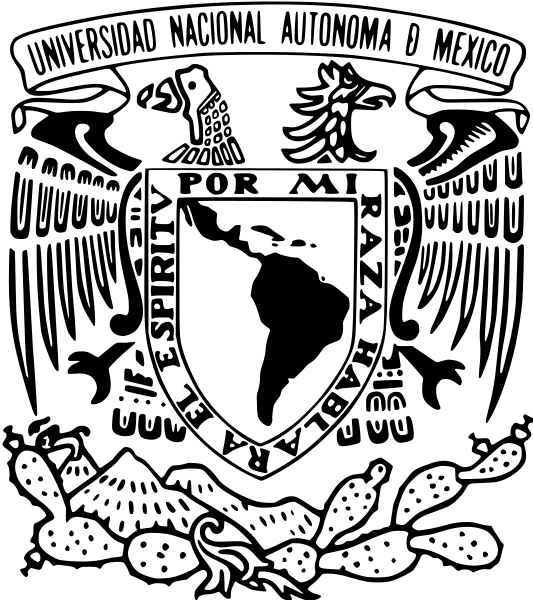
\includegraphics[height=3.4cm]{../unam_logo.png}
    \end{center}
  \end{minipage}\hfill
  \begin{minipage}{10cm}
    \begin{center}
      \textbf{\Large Universidad Nacional Autónoma de México}\\[0.2cm]
      \textbf{\large Facultad de Ciencias}\\[0.2cm]
      \textbf{Organización y Arquitectura de Computadoras 2025-2}\\[0.4cm]
      \textbf{\Large Práctica 08}\\[0.1cm]
      \textbf{Docentes:}\\
      José Galaviz \hspace{1em} Ricardo Pérez \hspace{1em} Ximena Lezama\\[0.3cm]
      \textbf{Autores:}\\
      Fernanda Ramírez Juárez \quad Ianluck Rojo Peña\\[0.3cm]
      \textbf{Fecha de entrega:} Domingo 20 de abril de 2025
    \end{center}
  \end{minipage}\hfill
  \begin{minipage}{3cm}
    \begin{center}
      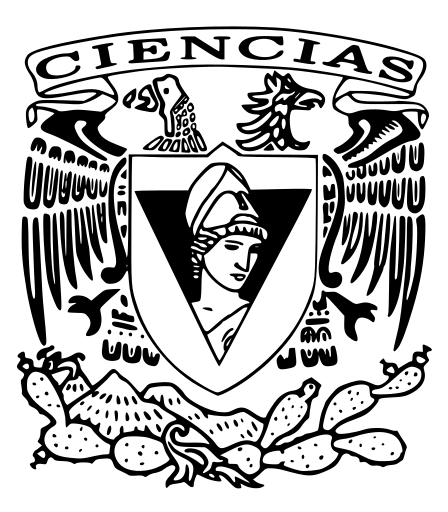
\includegraphics[height=3.4cm]{../fc_logo.png}
    \end{center}
  \end{minipage}
\end{center}

\bigskip
\hrule height 0.1pt
\bigskip

%------ Contenido -------- %
\section*{Ejercicios.}

\subsection*{Ejercicio 1.}

\textbf{¿Qué hace la rutina?}

El programa realiza la operación: $b^a$. Utiliza lo valores \texttt{a} que representa el exponente, y \texttt{b}, que representa la base.\\

Como agregado, la explicaci\'{o}n al flujo del programa es el siguiente:

\begin{enumerate}
\item En \texttt{main} cargmos los valores de \texttt{a} y \texttt{b} en los registros \texttt{\$a0} y \texttt{\$a1} e invocamos a la subrutina \texttt{mist\_1}, que se encarga de realizar el cálculo de elevar \texttt{b} a la potencia \texttt{a}.
\item Esta subrutina usa \texttt{loop\_1} que se repite \texttt{a} veces y en cada iteración llama a \texttt{mist\_0} con el que llevamos la cuenta de la multiplicación.
\item El valor inicial del acumulador es 1 y en cada iteración se multiplica por la base \texttt{b}, logrando así la operación \texttt{b * b * ... * b} (repetido \texttt{a} veces).
\item Cargamos el resultado final a \texttt{\$v0} y lo imprimimos junto con el mensaje \texttt{resultado} en consola.
\end{enumerate}

Teniendo en cuenta que los valores ya est\'{a}n establecidos con $a = 5$ y $b = 4$, la salida al correr el programa es:

\begin{verbatim}
El resultado es: 1024
\end{verbatim}

\newpage

\subsection*{Ejercicio 2.}

\begin{lstlisting}[style=cppstyle, caption={Código en C++ ~ Coeficiente binomial n en k utilizando la identidad de Pascal}]
  #include <iostream>
  #include <bits/stdc++.h>
  using namespace std;

  //Funcion que implementa el coeficiente binomial n en k utilizando la identidad de Pascal
  int coeficiente_binomial(int n, int k) {
    //Si k es mayor a n simplemente devolvemos 0
    if (k > n)
    return 0;
    //Caso base
    if (k == 0 || k == n)
    return 1;
    
    //Paso recursivo utilizando la identidad de Pascal
    return coeficiente_binomial(n - 1, k - 1) + coeficiente_binomial(n - 1, k);
  }

  int main() {
    int n, k;
    cout<< "Ingrese los valores para n, k: " << endl;
    cin >> n >> k;
    
    //Verificamos que n y k sean valores validos para calcular el coeficiente binomial
    if (n <= -1 || k <= 0) {
      cout << "[ERROR]: Los valores para n, k deben ser positivos.\n" << endl;
      return 0;
    }
    
    int r = coeficiente_binomial(n, k); //El resultado a de realizar el coeficiente
    cout << "El coeficiente binomial (" << n << " en " << k << ") es: " << r << endl;
  }

\end{lstlisting}

\newpage

\section*{Preguntas.}

\begin{enumerate}
\item ¿Qué es la Arquitectura Harvard Modificada (Modified Harvard Arquitecture)? ¿Cuáles son sus componentes?
  % -- Respuesta -- %

  La \textbf{Arquitectura Harvard Modificada} \textit{(Modified Harvard Architecture)} es una variante de la arquitectura Harvard clásica que combina características de esta última con elementos de la arquitectura von Neumann para mejorar la flexibilidad y eficiencia en sistemas modernos, sin sacrificar la ventaja principal de Harvard: el acceso simultáneo a ambas memorias a través de buses separados.\\
  
  \textbf{Diferencias:}
  
  \begin{itemize}
  \item \textbf{Harvard Clásica:} Separación total entre las memorias de instrucciones y de datos, con buses independientes y espacios de direcciones distintos.

  \item \textbf{Von Neumann:} Memoria unificada para instrucciones y datos, con un solo bus, lo que puede generar cuellos de botella.

  \item \textbf{Harvard Modificada:} Mantiene la separación física de memorias y buses, pero permite cierto grado de intercambio entre instrucciones y datos, especialmente para acceder a constantes almacenadas en la memoria de programa.
  \end{itemize}
  

  \textbf{Componentes principales de la arquitectura Harvard modificada.}
  
  \begin{itemize}
  \item \textbf{Memoria de Instrucciones \textit{(Program Memory)}:}
    
    Almacena el código ejecutable (programa). Suele ser de solo lectura (ROM/Flash) pero puede permitir acceso para lectura de datos.
    
  \item \textbf{Memoria de Datos \textit{(Data Memory)}:}
    
    Almacena variables y datos temporales. Normalmente es de lectura/escritura (RAM).
    
  \item \textbf{Buses separados:}
    
    Un bus para instrucciones (fetch) y otro para datos (load/store). Permite operaciones simultáneas (mayor velocidad que von Neumann).
    
  \item \textbf{Unidad de Intercambio \textit{(Data/Instruction Bridge)}:}

    Permite transferir datos entre memorias (como cargar constantes desde Flash a RAM). Es la principal mejora frente a la Harvard pura.
    
  \item \textbf{CPU \textit{(Unidad de Procesamiento Central)}:}
    
    Incluye ALU, registros y unidad de control. Puede acceder a ambas memorias en paralelo.
    
  \item \textbf{Periféricos y Puertos de Entrada/Salida:}
    
    Módulos adicionales para comunicación \textit{(UART, SPI, ADC, etc.)}.
    
  \end{itemize}
  
  \begin{figure}[H]
    \centering
    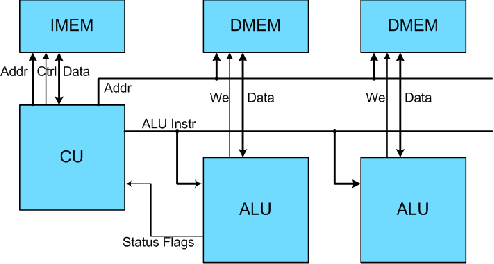
\includegraphics[width=0.6\textwidth]{image.png}
  \end{figure}

  \begin{itemize}
  \item \textit{Ventajas:}
    
    \begin{enumerate}[label=\arabic*)]
    \item Mayor velocidad al leer instrucciones y datos en paralelo.
      
    \item Flexibilidad para manejar constantes almacenadas en la memoria de programa.
      
    \item Ideal para sistemas en tiempo real (DSP, microcontroladores).
    \end{enumerate}
    
  \item \textit{Desventajas:}
    \begin{enumerate}[label=\arabic*)]
    \item Mayor complejidad en el diseño.
    \item Coste más alto que arquitecturas simples como von Neumann.
    \end{enumerate}
  \end{itemize}
  
  \textbf{Nota:}
  
  Esta arquitectura es popular en entornos embebidos donde el rendimiento y la optimización del acceso a memoria son esenciales, sin renunciar a cierta flexibilidad en el manejo de datos e instrucciones.
  
  En muchos sistemas modernos, se utiliza una variante conocida como arquitectura split-cache, donde hay una única memoria física pero con cachés separadas para instrucciones y datos, simulando una Harvard modificada en los niveles inferiores del procesador. También existen variantes que permiten ejecutar instrucciones desde memoria de datos o acceder a memoria de programa como si fuera de datos, aumentando la flexibilidad del sistema.
  
  \bigskip
  
\item En el contexto de las subrutinas, ¿Qué es el Wheeler Jump? Describe que pasos y para qué sirve el Wheeler Jump.
  % -- Respuesta -- %

  El \textbf{Wheeler Jump} es una técnica utilizada en programación de bajo nivel, especialmente en arquitecturas antiguas como la EDSAC (una de las primeras computadoras), para implementar subrutinas (funciones o procedimientos) de manera eficiente cuando no existían instrucciones nativas para manejar llamadas a subrutinas (como CALL y RET en CPUs modernas). Fue propuesto por \textit{David J. Wheeler}, uno de los pioneros de la computación.
  
  En sistemas primitivos sin pila de hardware ni instrucciones dedicadas para subrutinas, el Wheeler Jump permitía:

  \begin{enumerate}[label=\alph*)]
  \item Llamar a una subrutina guardando automáticamente la dirección de retorno.
    
  \item Retornar al punto de llamada después de ejecutar la subrutina.
    
  \item Era una solución ingeniosa para reutilizar código en entornos con recursos limitados.
  \end{enumerate}
  
  \textbf{Pasos del Wheeler Jump:}
  
  \begin{enumerate}[label=\arabic*)]
  \item Almacenamiento de la dirección de retorno:
    
    \begin{itemize}
    \item Antes de saltar a la subrutina, el programa modificaba la propia instrucción de salto dentro de la subrutina para que apuntase de vuelta a la dirección siguiente a la llamada.
      
    \item Esto se hacía copiando el contador de programa (PC) actual en el operando del salto.
    \end{itemize}
    
  \item Ejecución de la subrutina:
    
    \begin{itemize}
    \item La subrutina se ejecutaba normalmente.
    \item Al final, incluía una instrucción de salto modificada dinámicamente para retornar.
    \end{itemize}
    
  \item Retorno automático:
    
    \begin{itemize}
    \item Al llegar al salto modificado, la ejecución volvía a la instrucción siguiente a la llamada original.
    \end{itemize}
    
  \end{enumerate}
  
  Sin embargo, el \textbf{Wheeler Jump} contaba un ciertas limitaciones, comoq que dependía de auto-modificación de código, lo que hoy se considera mala práctica pues esto deriv en problemas de seguridad y mantenimiento. No permitía recursión, ya que solo se podía almacenar una dirección de retorno por subrutina, adem\'{a}s que acceder y escribir en memoria era lento comparado con registros o pilas.
  
  Fue posteriormente reemplazado por instrucciones como CALL/RET y el uso de pilas de hardware en arquitecturas siguietenes como x86 o ARM.
  
  No obstante, es un precursor clave de los mecanismos modernos de manejo de subrutinas. Demostró cómo resolver problemas complejos con recursos limitados, un principio aún relevante en sistemas embebidos.

  Hoy, el concepto persiste en formas más avanzadas, como los frames de pila en lenguajes de alto nivel, pero el Wheeler Jump sigue siendo un hito en la historia de la computación.

  \bigskip
  
\item ¿Por qué se causa la vulnerabilidad del Buffer Overflow (tambien llamado String Overflow)? ¿En C, cuál es el método que causaba este error?
  % -- Respuesta -- %

  \textbf{Buffer Overflow} \textit{(o String Overflow)} ocurre cuando un programa escribe datos en un buffer (espacio de memoria reservado) más allá de su capacidad asignada, sobrescribiendo áreas adyacentes de la memoria. Esto puede corromper datos, alterar el flujo de ejecución del programa o incluso permitir la ejecución de código malicioso.\\
  
  \textbf{Causas del Buffer Overflow:}

  \begin{itemize}
  \item \textbf{Falta de verificación de límites.}
    
    En lenguajes como C y C++, funciones que manejan buffers \textit{(como strcpy, gets, scanf)} no verifican automáticamente el tamaño del dato copiado. Si el dato es más grande que el buffer, se produce un overflow.
    
  \item \textbf{Organización de la memoria.}

    En la pila (stack), los buffers locales comparten espacio con: variables locales, la dirección de retorno de funciones, datos de control del programa. Un desbordamiento puede sobrescribir la dirección de retorno, redirigiendo la ejecución del programa.
    
  \item \textbf{Arquitectura de pila (Stack).}
    
    En C, las variables locales y la dirección de retorno de funciones se almacenan en la pila (stack). Si un buffer local se desborda, puede sobrescribir la dirección de retorno, permitiendo a un atacante redirigir la ejecución a código malicioso.

  \end{itemize}
  
  \textbf{Funciones inseguras en C:}
  
  \begin{table}[H]
    \centering
    \resizebox{\textwidth}{!}{ % Ajusta la tabla al ancho del documento
      \begin{tabular}{| m{8cm} | m{8cm} |}
        \hline
        \textbf{Función} & \textbf{Riesgo principal} \\ \hline
        \texttt{strcpy}  & Copia una cadena sin verificar l\'{i}mites. Riesgo de sobrescritura. \\ \hline
        \texttt{gets}    & Lee entrada del usuario sin límite de tamaño. Vulnerable a overflow. (Eliminada en C11) \\ \hline
        \texttt{strcat}  & Concatena sin verificar espacio restante en el buffer. Puede causar overflow. \\ \hline
        \texttt{scanf} con \texttt{\%s} & Sin especificar tamaño (\texttt{\%64s}) puede desbordar el buffer. \\ \hline
        \texttt{sprintf} & No verifica tamaño del buffer destino. Mejor usar \texttt{snprintf}. \\ \hline
      \end{tabular}
    }
  \end{table}
  
\end{enumerate}
\end{document}
